\section {Résultats obtenus}

Tous les tests ont été réalisés sur la machine hôte \texttt{worf} de
la salle 203 décrite ci-après~:
\begin{itemize}
\item NVIDIA GF100GL Quadro 4000
\item Intel Xeon E7 v2/Xeon E5 v2/Core i7
\item Deux noeuds NUMA~:
  \begin{itemize}
  \item cache L3 15 MB
  \item 6 coeurs physiques avec hyperthreading~:
    \begin{itemize}
    \item cache L2 256 KB
    \item L1d 32 KB
    \item L1i 32 KB
    \end{itemize}
  \end{itemize}
\end{itemize}
On pourra retrouver la sortie de la commande \texttt{lstopo} en
annexes (figure~\ref{fig:lstopo}). Nous exécutons chaque méthode 5
fois puis nous faisons une moyenne des 5 mesures de temps. L'unité des
mesures de temps est toujours le milliseconde.

\subsection{Comparaison des algorithmes séquentiels}

\begin{figure}[!ht]
  \center{
    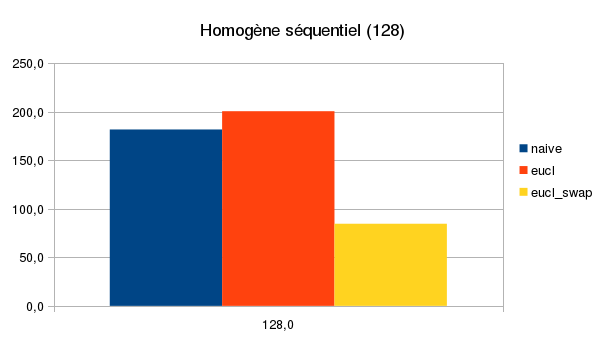
\includegraphics[width=10cm]{images/homoseq128.png}
  }
  \caption{}
  \label{fig:homoseq128}
\end{figure}

\begin{figure}[!ht]
  \center{
    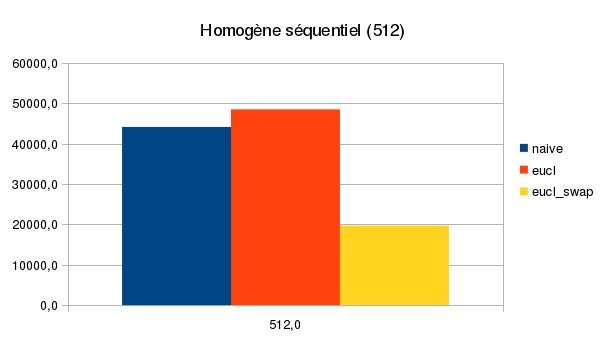
\includegraphics[width=10cm]{images/homoseq512.png}
  }
  \caption{}
  \label{fig:homoseq512}
\end{figure}

\begin{figure}[!ht]
  \center{
    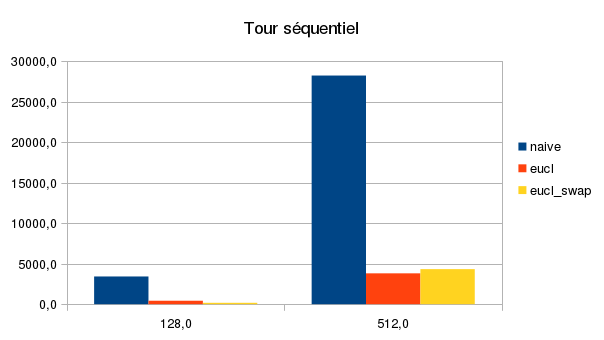
\includegraphics[width=10cm]{images/tourseq.png}
  }
  \caption{}
  \label{fig:tourseq}
\end{figure}

\subsubsection{Calcul naïf \textit{versus} division euclidienne}

La version qui utilise des divisions euclidiennes
\texttt{compute\_eucl} est 1,1 fois plus lente
(figure~\ref{fig:homoseq128} et~\ref{fig:homoseq512}) que la version
naïve \texttt{compute\_naive} pour les configurations homogènes. Cela
parait normal car les valeurs dans les cases à l'initialisation ne
dépassent pas 5. Ici, l'utilité de faire une division euclidienne est
limité.
\medskip

En revanche, pour le cas où on place un tas de 100000 grains au
centre, la version avec division euclidienne est 7 à 8 fois plus
rapide car on réduit le nombre d'itération nécessaire pour arriver à
stabilisation (figure~\ref{fig:tourseq}).

\subsubsection{Suppression des mauvaises prédictions de branchement}
\label{sec:predict}

La suppression de la condition qui vérifie si la valeur d'une case est
supérieure à la taille maximale d'un tas de sable améliore les
performances d'un facteur 3 environ pour la fonction
\texttt{compute\_eucl\_swap}.
\medskip

Grâce à l'optimisation de la section~\ref{sec:predict}, notre solution
\texttt{compute\_omp\_swap} qui limite les accès en écriture sur les
cases voisines est jusqu'à 2,5 fois plus rapide que les autres
méthodes séquentielles pour le cas homogène
(figure~\ref{fig:homoseq128} et~\ref{fig:homoseq512}). Sans la
suppression de la boucle, cette méthode est plus lente que les autres.

\subsubsection{Vectorisation et détection des zones stables}

Pour la méthode qui vectorise les calculs, nous n'avons pas obtenus
les performances espérées. La gestion des différents registres prend
plus de temps que d'effectuer 4 calculs. Cependant peut-être qu'avec
des registre de 512 bits (AVX) nous aurions obtenus de meilleurs
résultats. En revanche, les calculs sont corrects.

La version qui détecte les zones stable ne donne aussi pas de bons
résultats en plus d'avoir quelques bugs.

\subsubsection{Version OpenCL}
\label{sec:res-opencl}

La version OpenCL sur GPU donne aussi des résultats décevant (speed-up
de 0,3 pour la matrice de dimension 128 par 128 et 1,3 pour celle de
512 par 512). Cela est en partie du à la détection de la terminaison
de l'algorithme.

\subsection{Synchronisation toute les $p$-irérations}

Notre méthode \texttt{compute\_omp\_iter} n'est pas entièrement
fonctionnelle. Les résultats sont correctes mais aucun gain de temps
n'est à relever.

\subsection{Algorithmes multi-threads}

Pour le calcul du speed-up, nous prenons toujours comme temps de référence le
meilleur temps séquentiel pour le cas de figure étudié.
\bigskip

Sur les figures~\ref{fig:homopar128}, \ref{fig:homopar512},
\ref{fig:tourpar128}, et \ref{fig:tourpar512} on peut voir que la
méthode \texttt{compute\_omp} est plus lente que la méthode
\texttt{compute\_omp\_swap}. Cela peut s'expliquer par le surplus de
temps s'engendre l'étape de rapatriement des données dans la matrice
partagée, nécessaire après chaque itération.
\medskip

Les pics de speed-up correspondent aux exécutions avec un nombres de
threads multiples du nombres de lignes à traiter ($DIM-2$). Nous
pouvons voir l'intérêt de découper la matrice en morceaux égaux pour
tous les threads.
\medskip

Sur les figures~\ref{fig:homopar512} et~\ref{fig:tourpar512} nous
pouvons voir que pour une matrice de dimension 512 par 512, le speed-up
maximal de 8 est atteint pour un nombre de threads égal à 10. Ce
chiffre est rassurant car c'est le nombre maximal de coeur physiques qu'on peut
soliciter de la machine \texttt{worf} tout en ayant réparti le travail
équitablement en morceaux de matrice.
\medskip

Pour la matrice de taille 128, le speed-up maximal de 3 est atteint
pour une exécution avec 6 threads. Nous pouvons nous demander pourquoi
9 threads ne représente pas le nombre de threads idéal, car dans ce
cas nous solicitons plus de coeurs physiques tout en répartissant
mieux les lignes de la matrices. Le problème est que pour une telle
taille de matrice, l'exécution de l'algorithme est très courte~:
quelques dizaines de millisecondes. Ainsi, avec un nombre de threads
trop important, le programme passe plus de temps à synchroniser tous
ces threads qu'à calculer.
\medskip

\begin{figure}[!ht]
  \center{
    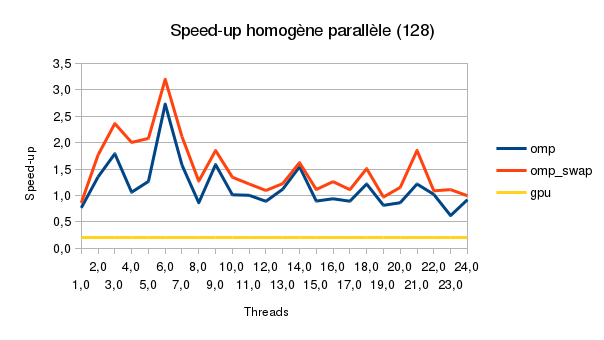
\includegraphics[width=10cm]{images/homopar128.png}
  }
  \caption{}
  \label{fig:homopar128}
\end{figure}

\begin{figure}[!ht]
  \center{
    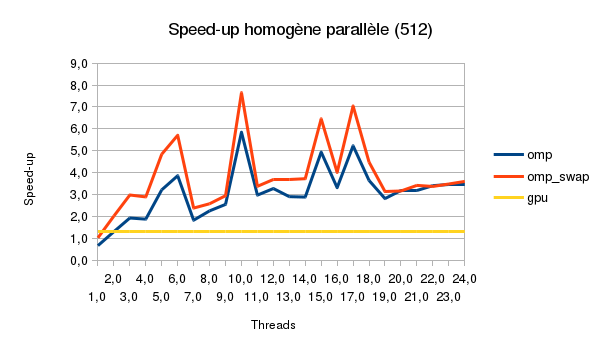
\includegraphics[width=10cm]{images/homopar512.png}
  }
  \caption{}
  \label{fig:homopar512}
\end{figure}

\begin{figure}[!ht]
  \center{
    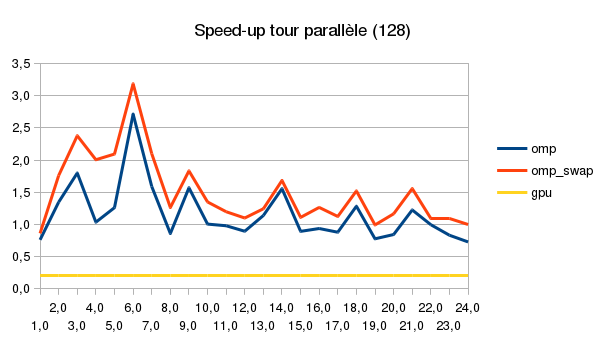
\includegraphics[width=10cm]{images/tourpar128.png}
  }
  \caption{}
  \label{fig:tourpar128}
\end{figure}

\begin{figure}[!ht]
  \center{
    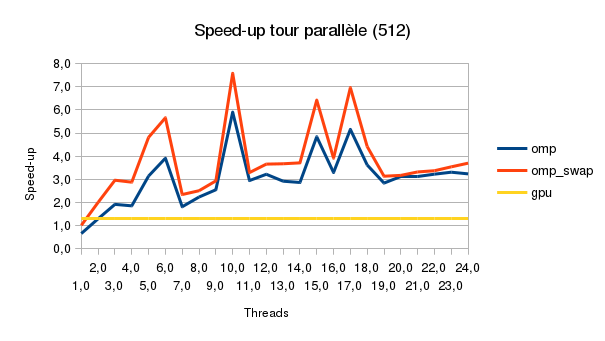
\includegraphics[width=10cm]{images/tourpar512.png}
  }
  \caption{}
  \label{fig:tourpar512}
\end{figure}
